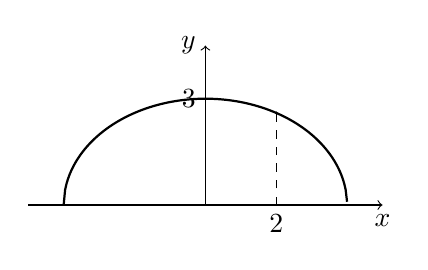
\begin{tikzpicture}[scale=0.45]
    \draw[->] (-5,0) -- (5,0) node[below] {$x$};
    \draw[->] (0,0) -- (0,4.5) node[left] {$y$};

    \draw[thick, domain=-4:4, samples=200] plot (\x,{3*sqrt(1-\x*\x/16)});
    \draw[thick] (-4,0) -- (4,0);

    \draw[dashed] (2,0) -- (2,{3*sqrt(1-4/16)});
    \fill (2,{3*sqrt(1-4/16)}) circle (1.2pt);

    \node[below] at (2,0) {$2$};
    \node[left] at (0,3) {$3$};
\end{tikzpicture}
